\chapter{Inequações}

As resoluções das inequações utilizam as propriedades de ordem $<$ dos números reais listadas abaixo.


\begin{obs}\index{Ordem!propriedades da relação de}\index{Propriedades!da relação de ordem}
\textbf{Propriedades da relação de ordem:} Dados $a,b,c \in \R$ temos que:
\begin{enumerate}[P1)]
\item \textbf{Adição:} $a < b \Leftrightarrow a+c < b+c$;
\item \textbf{Subtração:} $a < b \Leftrightarrow a-c < b-c$;
\item \textbf{Multiplicação por número positivo $c>0$:} $a<b \Leftrightarrow ac<bc$;
\item \textbf{Divisão por número positivo $c>0$:} $a<b \Leftrightarrow \frac{a}{c}<\frac{b}{c}$;
\item \textbf{Multiplicação por número negativo $c<0$:} $a<b \Leftrightarrow ac>bc$;
\item \textbf{Divisão por número negativo $c<0$:} $a<b \Leftrightarrow \frac{a}{c}>\frac{b}{c}$;
\end{enumerate}

Estas propriedades são validas quando usamos quaisquer dos sinais $<, \;\leq, \; >$ ou $\geq$.
\end{obs}

% \begin{obs}\index{Ordem!propriedades da relação de}\index{Propriedades!da relação de ordem}
% \textbf{Propriedades da relação de ordem:} Dados $x, y, z \text{ e } w \in \R$ temos que:
% \begin{enumerate}
% \item Se $x \leq y$ e $z \leq w$ então $x+z \leq y+w$.
% \item Se $0 \leq x \leq y$ e $0 \leq z \leq w$ então $0 \leq xz \leq yw$.
% \item $x < y \Leftrightarrow x+z < y+z$;
% \item $z>0 \Leftrightarrow z^{-1}>0$;
% \item $z>0 \Leftrightarrow -z> 0$;
% \item $z>0 \text{ e } x<y \Leftrightarrow xz<yz$;
% \item $z<0 \text{ e } x<y \Leftrightarrow xz>yz$;
% \item $0<x<y \Rightarrow 0< \dfrac{1}{y} < \dfrac{1}{x}$.
% \end{enumerate}
% \end{obs}

 \section{Inequações de 1º grau}
 
\begin{obs}
  As inequações do 1º grau possuem uma das seguintes formas gerais
 \begin{eqnarray*}
 ax+b \leq 0 \\
 ax+b < 0 \\
 ax+b \geqslant 0 \\
 ax+b >0 
 \end{eqnarray*}  
 para certos $a, b \in \R$ dados, com $a \neq 0$.
\end{obs}
  
 A principal diferença entre as equações de 1º grau e as inequações de 1º grau é que a equação possui uma única solução enquanto que a inequação possui, em geral, infinitas soluções, na forma de um intervalo real.
 
 \begin{exem} 
 $4x + 8 > 0$:
 
\begin{equation*}
4x + 8 > 0 \Leftrightarrow 4x > -8 \Leftrightarrow x > \frac{-8}{4} \Leftrightarrow x > -2.
\end{equation*}
 
 Portanto, o conjunto solução desta inequação pode ser representado pelo intervalo $\left(-2, +\infty \right)$ ou pelo conjunto $S=\{x \in \R \mid x > -2\}$. 
 
 Esta inequação tem o sinal ($>$) de maior, que representa uma desigualdade estrita, por este motivo $-2$ não faz parte do conjunto solução, portanto na representação em termos de intervalo temos um intervalo aberto em $-2$.
 \end{exem}
 
 \begin{exem} 
 $-x-3 \leq -4$:
\begin{equation*}
-x-3 \leq -4 \Leftrightarrow -x \leq -4 + 3 \Leftrightarrow -x \leq -1 \Leftrightarrow -x \leq -1 \ \ \cdot (-1) \Leftrightarrow x \geqslant 1.
\end{equation*}
 
 Como o $x$ estava negativo tivemos que multiplicar a inequação toda por $-1$. Mas precisamos cuidar porque quando multiplicamos uma inequação por um número negativo mudamos a desigualdade. Por isso obtemos como solução $x \geqslant 1$.
 
  O conjunto solução desta inequação pode ser representado pelo intervalo $\left[1, \infty \right)$ ou pelo conjunto $S=\{x \in \R \mid x \geqslant 1\}$. 
  
  Esta inequação tem o sinal ($\leq$) de menor ou igual, logo vale também a igualdade, por este motivo $1$ faz parte do conjunto solução, portanto na representação em termos de intervalo temos um intervalo fechado em $1$.
 \end{exem}
 
 % \begin{exem} 
 % $3x+2 \geqslant 5x-2$
 % \begin{eqnarray*}
 % 3x+2 & \geqslant & 5x-2 \\
 % 3x - 5x & \geqslant & -2-2 \\
 % -2x & \geqslant & -4 \ \ \cdot (-1) \\
 % 2x & \leq & 4 \\
 % x & \leq & \frac{4}{2} \\
 % x & \leq & 2
 % \end{eqnarray*}
 
 % Conjunto solução: $S=\{x \in \R \mid x \leq 2\}$.
 % \end{exem}
 
%   \begin{exem} 
%   $5x +1 > 3x - 5$
%   \begin{eqnarray*}
%   5x +1 &>& 3x - 5 \\
%   5x - 3x &>& -5 - 1 \\
%   2x &>& -6 \\
%   x &>& \frac{-6}{2} \\
%   x &>& -3
%   \end{eqnarray*}
%   Conjunto solução $S=\{x \in \R \mid x > -3\}$.
%  \end{exem}
 
%  \begin{exem} 
%  $3x - \dfrac{1}{3} < \dfrac{1}{2}$
 
%  \begin{eqnarray*}
%   3x - \dfrac{1}{3} &<& \dfrac{1}{2} \\
%   3x  &<& \dfrac{1}{2} + \dfrac{1}{3} \\
%   3x  &<& \dfrac{3 + 2}{6} \\
%   x  &<& \dfrac{\frac{5}{6}}{3} \\
%   x  &<& \dfrac{5}{6 \cdot 3} \\
%   x  &<& \dfrac{5}{18} \\
%   \end{eqnarray*}
  
%   Conjunto solução $S= \left\{x \in \R \mid x < \dfrac{5}{18} \right\}$.
%  \end{exem}
 
 %  \begin{exem} 
 % $\dfrac{x}{4} + \dfrac{1}{3} \geqslant \dfrac{5}{3}$
 % \begin{eqnarray*}
 %  \dfrac{x}{4} + \dfrac{1}{3} & \geqslant & \dfrac{5}{3} \\
 %  \dfrac{x}{4} & \geqslant & \dfrac{5}{3} - \dfrac{1}{3} \\
 %  x & \geqslant & \dfrac{4}{3} \cdot 4 \\
 %  x & \geqslant & \dfrac{16}{3}
 %  \end{eqnarray*}
 %  Conjunto solução: $S= \left\{x \in \R \mid x \geqslant \dfrac{16}{3} \right\}$.
 % \end{exem}
 
 \begin{exem}
 $\dfrac{3x+2}{2} - 3 \geqslant \dfrac{1}{4} - 2x$ 
 \begin{eqnarray*}
  \dfrac{3x+2}{2} - 3 &\geqslant & \dfrac{1}{4} - 2x \\
  \dfrac{2(3x+2)}{4} - \dfrac{12}{4} &\geqslant & \dfrac{1}{4} - \dfrac{8x}{4} \\
  \dfrac{6x+4}{4} + \dfrac{8x}{4} &\geqslant & \dfrac{1}{4} + \dfrac{12}{4} \\
  \dfrac{14x+4}{4}  &\geqslant & \dfrac{13}{4} \\
  14x  &\geqslant & 13 - 4\\
  x  &\geqslant & \dfrac{9}{14}\\
  \end{eqnarray*}
  Conjunto solução: $S= \left\{x \in \R \mid x \geqslant \dfrac{9}{14} \right\}$.
 \end{exem}
 
% \begin{exem}
% $\dfrac{1-2x}{3} + \dfrac{x-2}{6} > \dfrac{x+3}{2} - 1$
%   \begin{eqnarray*}
%   \dfrac{1-2x}{3} + \dfrac{x-2}{6} &>& \dfrac{x+3}{2} - 1 \\
%   \dfrac{2(1-2x)}{6} + \dfrac{x-2}{6} &>& \dfrac{3(x+3)}{6} - \dfrac{6}{6} \\
%   \dfrac{2 - 4x}{6} + \dfrac{x-2}{6} &>& \dfrac{3x+9}{6} - \dfrac{6}{6} \\
%   \dfrac{2}{6}- \dfrac{4x}{6}+ \dfrac{x}{6}- \dfrac{2}{6} &>& \dfrac{3x}{6}+ \dfrac{9}{6} - \dfrac{6}{6} \\
%   - \dfrac{4x}{6} + \dfrac{x}{6} - \dfrac{3x}{6} &>& \dfrac{9}{6} - \dfrac{6}{6} \\
%   \dfrac{-4x+x-3x}{6} &>& \dfrac{9-6}{6} \\
%   \dfrac{-6x}{6} &>& \dfrac{3}{6} \\
%   -x &>& \dfrac{1}{2} \cdot(-1)\\
%    x &<& \dfrac{-1}{2} \\
%   \end{eqnarray*}
 
%  Conjunto solução: $S=\left\{x \in \R \mid x < \dfrac{-1}{2} \right\}$.
% \end{exem}

% \begin{exem}
% $-6 \leqslant -2(x-3) \leqslant 3$

% Esta inqueção tem duas possíveis formas de resolver, vamos colocar as duas para que você possa escolher a que considerar mais fácil.

% 1ª Forma:
%  \begin{eqnarray*}
%    -6 \leqslant & -2(x-3) & \leqslant 3 \\
%    -6 \leqslant & -2(x-3) & \leqslant 3 \cdot (-1)\\
%    6 \geqslant & 2(x-3) & \geqslant -3 \\
%    -3 \leqslant & 2x - 6 & \leqslant 6 \\
%    -3+6 \leqslant & 2x & \leqslant 6+6 \\
%    \dfrac{3}{2} \leqslant & x & \leqslant \dfrac{12}{2} \\
%    \dfrac{3}{2} \leqslant & x & \leqslant 6
%  \end{eqnarray*}
 
   
% 2ª Forma:
%  \begin{eqnarray*}
%     -6 \leqslant & -2(x-3) & \leqslant 3 \\
%    -6 \leqslant & -2x + 6 & \leqslant 3 \\
%    -6-6 \leqslant & -2x & \leqslant 3-6  \\
%    -12 \leqslant & -2x & \leqslant -3 \cdot (-1) \\
%    12 \geqslant & 2x & \geqslant 3 \\
%    \dfrac{3}{2} \leqslant & x & \leqslant \dfrac{12}{2} \\
%    \dfrac{3}{2} \leqslant & x & \leqslant 6
%  \end{eqnarray*}
      
%   Conjunto solução $S= \left\{x \in \R \mid \dfrac{3}{2} \leqslant x \leqslant 6 \right\}$.

% \end{exem} 

% \begin{exem}
% $-5 \leqslant \dfrac{-3x + 5}{4} \leqslant 4$
  
%   \begin{eqnarray*}
%   -5 \leqslant & \dfrac{-3x + 5}{4} & \leqslant  4 \\
%    -5 \cdot 4  \leqslant & -3x + 5 & \leqslant 4 \cdot 4 \\
%    -20 - 5  \leqslant & -3x & \leqslant 16 - 5 \\
%    -25  \leqslant & -3x & \leqslant 11  \ \ \cdot(-1) \\
%    25  \geqslant & 3x & \geqslant -11 \\
%    \dfrac{-11}{3}  \leqslant & x & \leqslant \dfrac{25}{3}
%  \end{eqnarray*}
 
      
%   Conjunto solução $S= \left\{x \in \R \mid \dfrac{-11}{3} \leqslant x \leqslant \dfrac{25}{3} \right\}$.
% \end{exem}


 \section{Sinal do binômio \texorpdfstring{$ax+b$}{ax+b}}

Considere a expressão da forma $ax+b$, com constantes $a,b\in\R$, $a\neq 0$, e uma variável real $x$. Dependendo do valor de $x$ tem-se:
\begin{align*}
    ax+b&>0 & \mbox{ou} && ax+b&=0 & \mbox{ou} && ax+b&<0
\end{align*}

%pode assumir valor numérico positivo, negativo ou nulo, dependendo da escolha do valor de $x$.
Por exemplo, considere o binômio $3x-15$.

Se $x=6$ então $3(6)-15=3>0$.

Se $x=5$ então $3(5)-15=0$

Se $x=4$ então $3(4)-15=-3<0$.

A raiz do binômio $ax+b$ é a solução da equação $ax+b=0$, ou seja, $r=-\frac{b}{a}$. Estudar o sinal do binômio é averiguar quando $ax+b>0$ ou $ax+b<0$.

\begin{obs}
    Seja $r$ a raiz do binômio $ax+b$.
    \begin{itemize}
        \item Se $a>0$ então 
    $%\begin{equation*}
        \left\{
        \begin{matrix}
            ax+b>0 \Leftrightarrow x>-\frac{b}{a}=r\\
            ax+b<0 \Leftrightarrow x<-\frac{b}{a}=r.
        \end{matrix}
        \right.
    $%\end{equation*}
    
    Isto é interpretado na reta real da seguinte forma:
    \begin{signtbl}{1}{1}
        \linelabel{1}{$ax+b$}
        \numbernode{r}{1}{1}
        \signs{1}{-1,1}
    \end{signtbl}   

    \item Se $a<0$ então
    $
        \left\{
        \begin{matrix}
            ax+b>0 \Leftrightarrow x<-\frac{b}{a}=r\\
            ax+b<0 \Leftrightarrow x>-\frac{b}{a}=r.
        \end{matrix}
        \right.
    $

    Isto é interpretado na reta real da seguinte forma:
    \begin{signtbl}{1}{1}
        \linelabel{1}{$ax+b$}
        \numbernode{r}{1}{1}
        \signs{1}{1,-1}
    \end{signtbl} 
    \end{itemize}
\end{obs}

\begin{exem}
    Estude o sinal do binômio $-4x-6$.

    A raiz do binômio é $x=\frac{6}{-4}=-\frac{3}{2}$. Na reta real, temos:
    \begin{signtbl}{1}{1}
        \linelabel{1}{$-4x-6$}
        \numbernode{-\frac{3}{2}}{1}{1}
        \signs{1}{1,-1}
    \end{signtbl} 

    Assim,
    \begin{itemize}
        \item Para $x=-\frac{3}{2}$, o valor numérico do binômio é igual à zero;
        \item Para $x<-\frac{3}{2}$, o valor numérico do binômio é positivo;
        \item Para $x>-\frac{3}{2}$, o valor numérico do binômio é negativo.
    \end{itemize}
\end{exem}

%Queremos entender os intervalos da reta tal que 

\section{Inequação produto e quociente}

O estudo do sinal permite resolver inequações que envolvam produto e quociente de binômios.

\begin{exem}
    Resolva a inequação $(2x-1)(x+4)>0$.

    Para resolver esta equações, inicialmente fazemos o estudo do sinal dos binômios $2x-1$ e $x+4$:
    \begin{signtbl}{1}{1}
        \linelabel{1}{$2x-1$}
        \numbernode{\frac{1}{2}}{1}{1}
        \signs{1}{-1,1}
    \end{signtbl}
    \begin{signtbl}{1}{1}
        \linelabel{1}{$x+4$}
        \numbernode{-4}{1}{1}
        \signs{1}{-1,1}
    \end{signtbl}

    Em seguida, faremos o quado-produto (ou ``varal-produto'') a qual busca-se estudar o sinal do produto dos dois binômios

    \begin{signtbl}{3}{2}
        \linelabel{1}{$2x-1$}
        \numbernode{\frac{1}{2}}{1}{2}
        \signs{1}{-1,-1,1}
        \linelabel{2}{$x+4$}
        \numbernode{-4}{2}{1}
        \signs{2}{-1,1,1}
        \linelabel{3}{$(2x-1)(x+4)$}
        \numbernode{\frac{1}{2}}{3}{2}
        \numbernode{-4}{3}{1}
        \signs{3}{1,-1,1}
        \intervalcolor{violet}
        \intervalsign{3}{01}{1}
        \intervalsign{3}{10}{2}
    \end{signtbl}

    A solução da inequação é $S=(-\infty,-4)\cup(\frac{1}{2},+\infty)$.
\end{exem}

\begin{exem}
    Resolva a inequação $(x+1)(-x+2)\geq 0$.

    Podemos fazer a o estudo do sinal diretamente no quado-produto.

    \begin{signtbl}{3}{2}
        \linelabel{1}{$x+1$}
        \numbernode{-1}{1}{1}
        \signs{1}{-1,1,1}
        \linelabel{2}{$-x+2$}
        \numbernode{2}{2}{2}
        \signs{2}{1,1,-1}
        \linelabel{3}{$(x+1)(-x+2)$}
        \numbernode{-1}{3}{1}
        \numbernode{2}{3}{2}
        \signs{3}{-1,1,-1}
        \intervalcolor{violet}
        \intervalsign{3}{22}{1,2}
    \end{signtbl}

    A solução da inequação é $S=[-1,2]$.
\end{exem}

\begin{exem}
 $x^2-4x+3 \leqslant 0$
 
Para resolver uma inequação do 2º grau podemos escrevê-la como uma inequação produto. Calculando as raízes da equação do 2º grau:
\begin{equation*}
x^2-4x+3 = 0
\end{equation*}
 \begin{eqnarray*}
 x &=& \dfrac{-(-4) \pm \sqrt{(-4)^2 - 4 \cdot 1 \cdot 3}}{2 \cdot 1} \\
 x &=& \dfrac{4 \pm \sqrt{16 - 12}}{2} \\
 x &=& \dfrac{4 \pm \sqrt{4}}{2} \\
 x &=& \dfrac{4 \pm 2}{2} \\
 x' &=& \dfrac{4 + 2}{2} = 3 \ \\
 x'' &=& \dfrac{4 - 2}{2} = 1 \\
 \end{eqnarray*}
 
 Portanto, temos que $x^2-4x+3= (x-1) (x-3)$. Escrevendo o quadro-produto, temos que:
 \begin{signtbl}{3}{2}
        \linelabel{1}{$x-1$}
        \numbernode{1}{1}{1}
        \signs{1}{-1,1,1}
        \linelabel{2}{$x-3$}
        \numbernode{2}{2}{2}
        \signs{2}{1,1,-1}
        \linelabel{3}{$(x-1) (x-3)$}
        \numbernode{1}{3}{1}
        \numbernode{3}{3}{2}
        \signs{3}{1,-1,1}
        \intervalcolor{violet}
        \intervalsign{3}{22}{1,2}
\end{signtbl}
 
 Portanto, o conjunto solução desta inequação é o intervalo fechado $[1, 3]$, podemos também representar este conjunto solução por $S= \left\{ x \in \R \mid 1 \leqslant x \leqslant 3 \right\}$.
 \end{exem}

 \begin{exem}
 $-2x^2- 9x + 18 < 0$

  Resolvendo a equação $-2x^2- 9x + 18 = 0$ obtemos que as raízes são $-6$ e $\frac{3}{2}$. Assim, podemos escrever
\begin{equation*}
-2x^2- 9x + 18 = -2 (x+6) (x - \frac{3}{2}) = (x+6) (-2x +3). 
\end{equation*}

A escolha da última equação simplifica o quadro-produto.

 \begin{signtbl}{3}{2}
        \linelabel{1}{$x+6$}
        \numbernode{-6}{1}{1}
        \signs{1}{-1,1,1}
        \linelabel{2}{$-2x+3$}
        \numbernode{\frac{3}{2}}{2}{2}
        \signs{2}{1,1,-1}
        \linelabel{3}{$(x+6) (-2x +3)$}
        \numbernode{-6}{3}{1}
        \numbernode{\frac{3}{2}}{3}{2}
        \signs{3}{-1,1,-1}
        \intervalcolor{violet}
        \intervalsign{3}{01}{1}
        \intervalsign{3}{10}{2}
\end{signtbl}
% \begin{table}[H]
%  \centering
%  \begin{tabular}{|c|c|c|c|} \hline
%  \rowcolor{gray}
%     & $(-\infty, -6)$ & $\left(-6, \dfrac{3}{2} \right)$ & $\left(\dfrac{3}{2}, \infty \right)$ \\ \hline
%                 $x+6$ & $-$             & $+$       & $+$ \\ \hline
%             $-2x + 3$ & $+$             & $+$       & $-$ \\ \hline
% $(x+6) \cdot (-2x + 3)$ & $-$             & $+$       & $-$ \\ \hline
%  \end{tabular}
%  \end{table}
 
 Portanto, o conjunto solução desta inequação é o conjunto $(-\infty, -6) \cup \left(\dfrac{3}{2}, \infty \right)$, podemos também representar este conjunto solução por $S= \left\{ x \in \R \mid x < -6 \text{ ou } x > \dfrac{3}{2} \right\}$.
 \end{exem}

 Por enquanto, não tratatemos do caso em que a o polinômio de 2º grau não tem solução real. Isto deve ser visto quando estudarmos as funções de 2º grau.


\begin{obs}
  As inequações quociente são inequações dadas por quocientes/razões de polinômios. Como por exemplo:
  \[\dfrac{p(x)}{q(x)} > 0\]
  onde $p(x)$ e $q(x)$ são polinômios na variável $x$, com $q(x) \neq 0$. 
  
  Aqui podemos trocar $>$ por $<$, $\leq$ ou $\geqslant$ e contínuamos com uma inequação.    
\end{obs}
 
 Lembramos que não existe divisão por zero, logo estas inequações estão definidas apenas no conjunto
  \[D= \{ x \in \R \mid  q(x) \neq 0\} \ . \]  
  %Este subconjunto $D$ dos números Reais no qual a inequação esta definida é chamado domínio da inequação. 
  
  O conjunto solução da inequação é necessariamente um subconjunto deste conjunto $D$.

\begin{exem}
    $\dfrac{2x-8}{-3x-6}<0$

    Vejamos inicialmente a restrição da solução. Como o denominador dever ser não nulo então $-3x-6\neq 0$, isto é, $x\neq -2$.

    Agora, fazemos o quadro de sinais dos binômios $2x-8$ e $-3x-6$:
    \begin{signtbl}{3}{2}
        \linelabel{1}{$2x-2$}
        \numbernode{4}{1}{2}
        \numbernode{4}{3}{2}
        \signs{1}{-1,-1,1}
        \linelabel{2}{$-3x-6$}
        \numbernode{-2}{2}{1}
        \numbernode{-2}{3}{1}
        \signs{2}{1,-1,-1}
        \intervalcolor{violet}
        \signs{3}{-1,1,-1}
        \linelabel{3}{$\frac{2x-8}{-3x-6}$}
        \intervalsign{3}{01}{1}
        \intervalsign{3}{10}{2}
\end{signtbl}

    Assim, a solução da inequação é $S=(-\infty,-2)\cup(4,+\infty)$.
\end{exem}

\begin{exem}
  $\dfrac{x^2+x+4}{x+1} \geq 4$

  Para resolver a inequação começamos colocando todos as espressões do lado esquerdo da equação e tomamos o minímo múltiplo comum das duas frações para poder efetuar a soma das frações.

  \[\frac{x^2+x+4}{x+1} -4 \geq 0 \Rightarrow
    \frac{x^2+x+4-4x-4}{x+1} \geq 0 \Rightarrow
    \frac{x^2 - 3x}{x+1} \geq 0
  \]
  
  Vamos determinar a restrição da solução. Neste caso para que a inequação esteja bem definida precisamos ter $x+1 \neq 0$ o que é satisfeito para $x \neq -1$. Portanto,
  \[D= \{x \in \R \mid x \neq -1\}.\]
  
  % Para resolver a inequação começamos tirando o minímo múltiplo comum das duas frações para poder efetuar a soma das frações, lembrando que quando o denominador não aparece ele é um.

  % \[4 - \frac{x^2+x+4}{x+1} \leq 0 \Rightarrow
  %   \frac{4x+4-x^2-x-4}{x+1} \leq 0 \Rightarrow
  %   \frac{-x^2 + 3x}{x+1} \leq 0
  %\]
  Podemos escrever $x^2 - 3x=x(x-3)$. %Em seguida, vamos fazer o $-x^2 + 3x=x(-x+3)$ e $x+1$ separadamente para poder fazer o estudo de sinal do quociente entre elas.
% \begin{equation*}
% x+1=0 \Leftrightarrow x= -1
% \end{equation*}
% \begin{equation*}
% -x^2 + 3x= 0 \Leftrightarrow x(-x+3)=0 \Leftrightarrow x=0 \ \ \text{ou} \ \ x=-3
% \end{equation*}
%Aqui alternativamente a tabela faremos o estudo de sinal da inequação quociente graficamente, que pode ser mais fácil para algumas pessoas visualizar o resultado.
Vejamos agora o quadro de sinais com as expressões $x$, $x-3$ e $x+1$:
\begin{signtbl}{4}{3}
        \linelabel{1}{$x$}
        \numbernode{0}{1}{2}
        \numbernode{0}{4}{2}
        \signs{1}{-1,-1,1,1}
        \linelabel{2}{$x-3$}
        \numbernode{3}{2}{3}
        \numbernode{3}{4}{3}
        \signs{2}{-1,-1,-1,1}
        \linelabel{3}{$x+1$}
        \numbernode{-1}{3}{1}
        \numbernode{-1}{4}{1}
        \signs{3}{-1,1,1,1}
        \intervalcolor{violet}
        \signs{4}{-1,1,-1,1}
        \linelabel{4}{$\frac{x(x - 3)}{x+1}$}
        \intervalsign{4}{12}{1,2}
        \intervalsign{4}{20}{3}
\end{signtbl}

 %   \begin{figure}[H]
 % \centering
 % 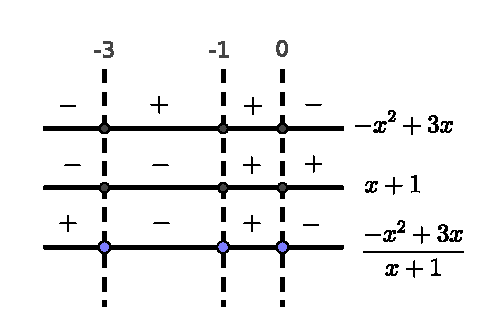
\includegraphics[width=8cm]{./cap_equacoes/figs/sinais}
 % \end{figure}

 Logo, pelo estudo de sinais acima, e considerando a restrição da inequação, obtemos o conjunto solução
\begin{equation*}
S= (-1, 0] \cup [3, +\infty).
\end{equation*}
 \end{exem}



\section{Sistema de inequações}

Algumas vezes, é necessário obter valores de $x$ que satisfazem duas ou mais inequações simultâneamente, o que denominamos \emph{sistema de inequações}. O conjunto solução de um sistema de inequações é a interseção dos conjuntos solução de cada inequação do sistema.

\begin{exem}
    $-1<2x-3\leqslant 3$

    Resolver esta inequação simultânea é equivalente à resolver o sistema:
    \begin{equation*}
    \left\{
        \begin{matrix}
            -1<2x-3\\
            2x-3\leqslant 3
        \end{matrix}
    \right.
    \end{equation*}

    A solução da primeira equação é $S_1=\{x\in\R \mid x>1\}=(1,+\infty)$ e da segunda equação é $S_2=\{x\in\R \mid x\leq 3\}=(-\infty,3]$. Fazendo a interseção das soluções:
    \begin{intervaloper}[3]{0}{4}
        \linelabel{1}{$S_1$}
        \linelabel{2}{$S_2$}
        \linelabel{3}{$S=S_1\cap S_2$}
        \dashes{1}{1}{3}
        \dashes{3}{1}{3}
        \interval{1}{10}{1}
        \interval{2}{02}{3}
        \intervalcolor{blue}
        \interval{3}{12}{1,3}
    \end{intervaloper}
    
    Logo, a solução geral do sistema é $S=S_1\cap S_2 = \{x\in\R \mid 1< x\leq 3\}=(1,3]$.
\end{exem}

\begin{exem}
    $3x+2<-x+3\leq x+4$

    Resolver esta inequação simultânea é equivalente à resolver o sistema:
    \begin{equation*}
    \left\{
        \begin{matrix}
            3x+2<-x+3\\
            -x+3\leq x+4
        \end{matrix}
    \right.
    \end{equation*}

    Assim, da 1ª equação temos
    \begin{equation*}
        3x+2<-x+3 \Rightarrow 4x<1 \Rightarrow x<\frac{1}{4}
    \end{equation*}
    e da 2ª equação
    \begin{equation*}
        -x+3\leq x+4 \Rightarrow -2x\leq 1 \Rightarrow x\geq -\frac{1}{2}.
    \end{equation*}

    Fazendo a interseção das soluções:
    \begin{intervaloper}[3]{-1}{1}
        \linelabel{1}{$S_1$}
        \linelabel{2}{$S_2$}
        \linelabel{3}{$S=S_1\cap S_2$}
        \dashes{-1/2}{1}{3}
        \dashes{1/4}{1}{3}
        \interval{1}{01}{1/4}
        \interval{2}{20}{-1/2}
        \intervalcolor{blue}
        \interval{3}{21}{-1/2,1/4}
    \end{intervaloper}
    
    Logo, a solução geral do sistema é $S=S_1\cap S_2 = \left[-\frac{1}{2}, \frac{1}{4} \right)$.
\end{exem}





 
%  \section{Inequações de 2º grau}
 
%  \begin{obs}
%   As inequações do 2º grau possuem uma das seguintes formas gerais
%  \begin{eqnarray*}
%  ax^2 + bx + c \leq 0 \\
%  ax^2 + bx + c < 0 \\
%  ax^2 + bx + c \geqslant 0 \\
%  ax^2 + bx + c >0 
%  \end{eqnarray*}  
%  para certos $a, b, c \in \R$ dados, com $a \neq 0$.
% \end{obs}
  
%  A principal diferença entre as equações de 2º grau e as inequações de 2º grau é que a equação, quando possui solução tem uma ou duas soluções, equanto que a inequação quando possui solução possui infinitas soluções, que representam um intervalo real ou a união de dois intervalos reais. 
 
%  Vejamos alguns exemplos de como resolver inequações do 2º grau, é importante ressaltar que para resolver inequações do 2º grau precisamos das técnicas de resoluções de equações do 2º grau, as quais foram apresentadas e exemplificadas anteriormente.
 
 
%  \begin{exem}
%  $x^2 + x - 20 \geqslant 0$
 
%  Resolvendo a equação $x^2 + x - 20 = 0$ obtemos que
% \begin{equation*}
% x^2 + x - 20  = (x+5) \cdot (x-4) . 
% \end{equation*}
 
%  Observemos que, $x+5> 0 \Leftrightarrow x> -5$ e que $x-4> 0 \Leftrightarrow x>4$. 
 
%  Portanto, temos três intervalos reais para analisar o sinal da inequação $x^2 + x - 20 \geqslant 0$, são eles $(-\infty, -5)$, $(-5, 4)$ e $(4, \infty)$. Para facilitar esta análise considere a seguinte tabela:

 
%  \begin{table}[H]
%  \centering
%  \begin{tabular}{|c|c|c|c|} \hline
%  \rowcolor{gray}
%                       & $(-\infty, -5)$ & $(-5, 4)$ & $(4, \infty,)$ \\ \hline
%                 $x+5$ & $-$             & $+$       & $+$ \\ \hline
%                 $x-4$ & $-$             & $-$       & $+$ \\ \hline
%  $(x+5) \cdot (x-4)$  & $+$             & $-$       & $+$ \\ \hline
%  \end{tabular}
%  \end{table}
 
%  Portanto, o conjunto solução desta inequação é o conjunto $(-\infty, -5] \cup [4, \infty)$, podemos também representar este conjunto solução por $S= \left\{ x \in \R \mid x \leqslant -5 \text{ ou } x \geqslant 4 \right\}$.
%  \end{exem}
 
 
 
%  \begin{exem}
%  $x^2 - 16 < 0$
 
%  \begin{eqnarray*}
%  x^2 - 16 < 0 \Leftrightarrow x^2 < 16 \Leftrightarrow \abs{x} < \sqrt{16} \Leftrightarrow -4 < x < 4
%  \end{eqnarray*}
 
% Portanto, o conjunto solução desta inequação é o conjunto $(-4, 4)$, podemos também representar este conjunto solução por $S= \left\{ x \in \R \mid -4 < x < 4 \right\}$. 
%  \end{exem}
 
%  \begin{exem}
%  $(x-2)^2 < 3x -2$
 
%  Simplificando a inequação obtemos:
%  \begin{eqnarray*}
%  (x-2)^2 < 3x -2 \Leftrightarrow x^2 -4x + 4 < 3x - 2 \Leftrightarrow x^2-4x-3x+4+2<0 \Leftrightarrow x^2-7x+6<0 \\
%  \end{eqnarray*}
%   Resolvendo a equação $x^2-7x+6= 0$ obtemos que
% \begin{equation*}
% x^2-7x+6 = (x-1) \cdot (x-6) . 
% \end{equation*}
 
%  Observemos que, $x-1> 0 \Leftrightarrow x>1$ e que $x-6> 0 \Leftrightarrow x >6$. 
 
%  Portanto, temos três intervalos reais para analisar o sinal da inequação $x^2-7x+6 < 0$, são eles $(-\infty, 1)$, $\left(1, 6 \right)$ e $\left(6, \infty\right)$. Para facilitar esta análise considere a seguinte tabela:
 
%  \begin{table}[H]
%  \centering
%  \begin{tabular}{|c|c|c|c|} \hline
%  \rowcolor{gray}
%     & $(-\infty, 1)$ & $\left(1, 6 \right)$ & $\left(6, \infty \right)$ \\ \hline
%                 $x-1$ & $-$             & $+$       & $+$ \\ \hline
%                 $x-6$ & $-$             & $-$       & $+$ \\ \hline
%   $(x-1) \cdot (x-6)$ & $+$             & $-$       & $+$ \\ \hline
%  \end{tabular}
%  \end{table}
 
%  Portanto, o conjunto solução desta inequação é o conjunto $(1 , 6)$, podemos também representar este conjunto solução por $S= \left\{ x \in \R \mid 1 < x < 6 \right\}$.
%  \end{exem}
 
%  \begin{exem}
%  $x^2-x+1>0$
 
%  Note que a equação $x^2-x+1= 0$ possui $\Delta= -3 < 0$ portanto esta equação não possui solução real. Neste caso para resolver a inequação $x^2-x+1>0$, podemos por exemplo utilizar o completamento de quadrados, com o qual obtemos que:

%  \begin{eqnarray*}
%  x^2-x+1>0 \Leftrightarrow \left(x - \dfrac{1}{2} \right)^2 + \dfrac{3}{4} > 0.
%  \end{eqnarray*}
%  Sabemos que $\left(x - \dfrac{1}{2} \right)^2 > 0$ para qualquer $x \in \R$, e que ao somar números positivos o resultado é um número positivo, com isso podemos concluir que $\left(x - \dfrac{1}{2} \right)^2 + \dfrac{3}{4} > 0$ para qualquer $x \in \R$. Portanto o conjunto solução da inequação $x^2-x+1>0$ é $S= \R= (-\infty, \infty)$.
 
%  Vale observar, aproveitando as contas acima, que a inequação $x^2-x+1<0$ não possui solução, logo para esta inequação temos $S= \emptyset$.
 
%  \end{exem}



%  \section{Inequações racionais}

% \begin{obs}
%   As inequações racionais são inequações dadas por quocientes/razões de polinômios. Como por exemplo:
%   \[\dfrac{p(x)}{q(x)} > 0\]
%   onde $p(x)$ e $q(x)$ são polinômios na variável $x$, com $q(x) \neq 0$. 
  
%   Aqui podemos trocar $>$ por $<$, $\leq$ ou $\geqslant$ e contínuamos com uma inequação.    
% \end{obs}
 
%  Lembramos que não existe divisão por $0$ (zero), logo estas inequações estão definidas apenas no conjunto
%   \[D= \{ x \in \R \mid  q(x) \neq 0\} \ . \]  
%   Este subconjunto $D$ dos números Reais no qual a inequação esta definida é chamado domínio da inequação. O conjunto solução da inequação é necessariamente um subconjunto do domínio da inequação.
  
%   Quando ambos os lados de uma inequação racional são não nulos, como por exemplo $\dfrac{p(x)}{q(x)} > 3$, um dos possíveis caminhos a se seguir na resolução da inequação é multiplicar ambos os lados da inequação por $q(x)$, mas para fazer isso corretamente é necessário levar em consideração o sinal de $q(x)$, o que nos força a quebrar a resolução em casos, daremos um exemplo de como fazer isso. Mas para evitar este tipo de problema temos como sugestão seguir os seguintes passos:
%   \begin{enumerate}[1)]
%   \item Mova todos os termos para o lado esquerdo da inequação, ficando com $0$ do lado direito;
%   \item Escreva a expressão resultante no lado esquerdo como uma única fração, com numerador e denominador fatorados;
%   \item Determine o domínio da inequação resultante;
%   \item Determine as raízes do numerador e denominador (quando for o caso) e use-os para definir os extremos dos intervalos;
%   \item Construa uma tabela, relacionando os sinais de cada fator em cada um dos intervalos, use esta tabela para fazer o estudo de sinal da inequação racional.
%   \item Determine a solução da inequação racional com base nas informações obtidas na tabela.
%   \end{enumerate}
 
% 	Após a realização dos dois primeiros passos listados acima, obtemos uma inequação de uma das seguintes formas:
% 	\begin{eqnarray}
% 	\dfrac{p(x)}{q(x)} \leq 0 \\
% 	\dfrac{p(x)}{q(x)} \geqslant 0
% 	\end{eqnarray}
% nas quais o lado direito é zero. Assim para chegar ao conjunto solução basta fazer a análise de sinal da expressão $\dfrac{p(x)}{q(x)}$, para isso consideramos os seguintes casos:

% Caso 1:	$\dfrac{p(x)}{q(x)} > 0$ se $p(x)$ e $q(x)$ tem o mesmo sinal, ou seja, nos seguintes conjuntos 
% \[ S_1= \{x \in \R \mid p(x)>0 \text{ e } q(x)>0 \} \]
% ou
% \[ S_2= \{x \in \R \mid p(x)<0 \text{ e } q(x)<0 \} \]
% logo o conjunto solução da inequação neste caso é $S= S_1 \cup S_2$.

% Caso 2:	$\dfrac{p(x)}{q(x)} < 0$ se $p(x)$ e $q(x)$ tem sinais opostos, ou seja, nos seguintes conjuntos 
% \[ R_1= \{x \in \R \mid p(x)>0 \text{ e } q(x)<0 \} \]
% ou
% \[ R_2= \{x \in \R \mid p(x)<0 \text{ e } q(x)>0 \} \]
% logo o conjunto solução da inequação neste caso é $S= R_1 \cup R_2$.
	
 
%  \begin{exem}
%   $4 - \dfrac{x^2+x+4}{x+1} \leq 0$
%   Antes de começar a resolver a inequação vamos determinar seu domínio. Neste caso para que a inequação esteja bem definida precisamos ter $x+1 \neq 0$ o que é satisfeito para $x \neq -1$. Portanto o domínio desta inequação é:
%   \[D= \{x \in \R \mid x \neq -1\} \ .\]
  
%   Para resolver a inequação começamos tirando o minímo múltiplo comum das duas frações para poder efetuar a soma das frações, lembrando que quando o denominador não aparece ele é um.

%   \[4 - \frac{x^2+x+4}{x+1} \leq 0 \Rightarrow
%     \frac{4x+4-x^2-x-4}{x+1} \leq 0 \Rightarrow
%     \frac{-x^2 + 3x}{x+1} \leq 0
%   \]
%   Agora vamos calcular os zeros de cada uma das equações $-x^2 + 3x$ e $x+1$ separadamente para poder fazer o estudo de sinal do quociente entre elas.
% \begin{equation*}
% x+1=0 \Leftrightarrow x= -1
% \end{equation*}
% \begin{equation*}
% -x^2 + 3x= 0 \Leftrightarrow x(-x+3)=0 \Leftrightarrow x=0 \ \ \text{ou} \ \ x=-3
% \end{equation*}

% Aqui alternativamente a tabela faremos o estudo de sinal da inequação quociente graficamente, que pode ser mais fácil para algumas pessoas visualizar o resultado.
% \begin{center}
%     \signtable[3]{-3,-1,0}{-1,1,1,-1}{-1,-1,1,1}{$-x^2+3x$}{$x+1$}{$\frac{-x^2+3x}{x+1}$}[2]
% \end{center}

%  %   \begin{figure}[H]
%  % \centering
%  % 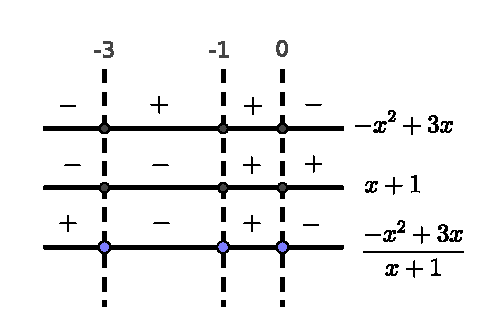
\includegraphics[width=8cm]{./cap_equacoes/figs/sinais}
%  % \end{figure}

%  Logo pelo jogo de sinais da figura acima, e considerando o domínio da inequação, obtemos
% \begin{equation*}
% S= [-3, -1) \cup [0, +\infty)
% \end{equation*}
%  como conjunto solução desta inequação.

%  \end{exem}

\begin{secExercicios}

\begin{exer}
   Resolva as inequações em $\R$:
    \begin{enumerate}[a)]
        \item $x + 1 \leq 7 - 3x < \dfrac{x}{2}-1$
        \item $3x+4 < 5 < 6-2x$
        \item $2-x<3x+2<4x+1$
        \item $(x-5)(3x-9)(-2x+8)<0$
        \item $-2x(x-1)(3x+4)<0$
        \item $\dfrac{x}{x-2}>3$
        \item $(2x-1)^3(x+2)>0$
        \item $(x-2)^2 \geq 0$
        \item $(x-\sqrt{2})(2x+3)(x-1)\geq0$
        \item $\dfrac{(2-5x)(x+1)}{(-x+3)}\leq 0$
        \item $\dfrac{x}{x+1} - \dfrac{x}{x-1} \geq 0$
        \item $\dfrac{2x}{x+2} > 2$
        \item $\dfrac{2}{x+1} + \dfrac{1}{x-1} \leq \dfrac{3}{x}$
    \end{enumerate}
\end{exer}

\begin{exer}
    Determine o os valores de $x$ no conjunto dos números naturais $\N$ que satisfazem
    \begin{equation*}
        5x-9<3x+1
    \end{equation*}
\end{exer}


\begin{exer}
    Determine o conjunto solução da inequação:
    \begin{equation*}
        \frac{x+1}{2}<5+x\leq \frac{2x-1}{4}.
    \end{equation*}
\end{exer}

\begin{exer}
    Resolva as inequações:
    \begin{enumerate}[a)]
        \item $(4x+5)^5<0$
        \item $(-3x-12)^4>0$
        \item $(x+6)^6\leq 0$
        \item $(x-2)^8(3-x)^5(4x+1)^7>0$
    \end{enumerate}
\end{exer}

\begin{exer}
    (Fuvest-SP) Resolva a inequação
    \begin{equation*}
        \frac{x^2-x-1}{\sqrt{x^2-3x}}\geq 0.
    \end{equation*}
\end{exer}

\begin{exer}
    Resolva os sistemas de inequações em $\R$:
    \begin{enumerate}[a)]
        \item  $\left\{
        \begin{matrix}
            3x-2 > 4x+1\\
            5x+1 \leq 2x-5
        \end{matrix}
    \right.$
        \item $\left\{
        \begin{matrix}
            5x-2 <0\\
            3x+1 \geq 4x-5\\
            x-3 \geq 0
        \end{matrix}
    \right.
    $
        \item $\left\{
        \begin{matrix}
            3x+2 \geq 5x - 2\\
            4x-1 > 3x-4\\
            3-2x < x-6
        \end{matrix}
    \right.$
        \item  $\left\{
        \begin{matrix}
            \dfrac{2x-5}{1-x} \leq -2\\
            \dfrac{x^2 + x + 3}{x+1} > x
        \end{matrix}
    \right.$
    \end{enumerate}
\end{exer}
\end{secExercicios}

%\subsection*{Respostas:}
%\shipoutAnswer